\newpage

\subsection{Аналитическое моделирование}

Введём следующие обозначения: \\
$\lambda_{\text{ф}_1}$ -- среднее значение суммарной интенсивности фонового потока запросов, выходящих из ОА, имитирующих работу рабочих станций, в канал; \\
$\lambda_{\text{ф}_1}\beta$ -- среднее значение интенсивности фонового потока запросов, проходящих через ОА, имитирующих работу сервера и дисков, где $\beta=\frac{1}{1 - P}$; \\
$\beta$ -- среднее количество проходов запроса по тракту процессор-диски за время одного цикла его обработки в системе; \\
$t_{\text{к}} = 0.5\cdot(t_{\text{к}_1} + t_{\text{к}_2})$ -- среднее значение времени обработки запроса в канале передачи данных, где $t_{\text{к}_1}$ и $t_{\text{к}_2}$ -- соответственно среднее время передачи запроса по каналу в прямом и обратном направлениях;
$n$ -- количество серверов, обслуживающих рабочие станции; \\
$m = \frac{1}{P_i}$ -- количество дисков в сервере, при условии, что все они одинаковые; \\
$P_i$ -- вероятность обращения к $i$-му диску сервера.\par\bigskip

При расчете используется приближённый итерационный алгоритм нахождения значения выходных характеристик рассматриваемой системы:
\begin{enumerate}

\item Определяем начальное значение для $\lambda_{\text{ф}_1}$: \\
 $$\lambda_{\text{ф}_1} = K_1min\left\{\frac{1}{2\cdot t_{\text{к}}};\frac{\text{С}}{\beta\cdot t_{\text{пр}}};\frac{1}{\beta\cdot P_i\cdot t_{\text{д}}}\right\}\cdot\frac{N - 1}{N}$$ \\
 $K_1$ принимает значения в диапазоне 0.995...0.99995.\par
 Определяем средние времена пребывания запроса в узлах системы (канале, процессоре, дисках): \\
 $$T_{\text{к}} = \frac{2\cdot t_{\text{к}}}{1 - 2\cdot\lambda_{\text{ф}_1}\cdot t_{\text{к}}}$$
 $$T_{\text{пр}} = \frac{\beta\cdot t_{\text{пр}}}{1 - (\beta\cdot\lambda_{\text{ф}_1}\cdot\frac{t_{\text{пр}}}{\text{С}})^{\text{С}}}$$
 $$T_{\text{д}} = \frac{\beta\cdot t_{\text{д}}}{1 - \beta\cdot P_i\cdot\lambda_{\text{ф}_1}\cdot t_{\text{д}}}$$
 
\item Определяем интенсивность фонового потока после очередной итерации:
 $$\lambda_{\text{ф}} = \frac{N - 1}{T_{\text{о}} + T_{\text{р}} + T_{\text{к}} + T_{\text{пр}} + T_{\text{д}}}$$
 
\item Сравниваем $\lambda_{\text{ф}_1}$ и $\lambda_{\text{ф}}$. Если $\frac{|\lambda_{\text{ф}_1} - \lambda_{\text{ф}}|}{\lambda_{\text{ф}}} < \Delta_1$, то переход на пункт 5, иначе на 4;

\item Определяем новое приближённое значение для $\lambda_{\text{ф}_1}$:
 $$\delta_1 = \frac{\lambda_{\text{ф}_1} - \lambda_{\text{ф}}}{K_2}$$
 $K_2$ принимает значения в диапазоне 10...1000.
 $$\lambda_{\text{ф}_1} = \lambda_{\text{ф}_1} - \delta_1$$
 Переход на пункт 2.
 
\item Определяем выходные результаты аналитической модели: \\
 $$T_{\text{цикла}} = T_{\text{о}} + T_{\text{р}} + T_{\text{к}} + T_{\text{пр}} + T_{\text{д}}$$
 $\lambda = \frac{N}{T_{\text{цикла}}}$
 Определяем загрузку основных узлов системы.\\ 
 Рабочей станции: $$\rho_{PC} = \frac{T_{\text{о}} + T_{\text{р}}}{T_{\text{цикла}}}$$
 Пользователя: $$\rho_{\text{польз}} = \frac{T_{\text{р}}}{T_{\text{цикла}}}$$
 Канала передачи данных: $$\rho_{\text{к}} = 2\cdot\lambda\cdot t_{\text{к}}$$
 Процессора: $$\rho_{\text{пр}} = \frac{\beta\cdot\lambda\cdot t_{\text{пр}}}{\text{С}}$$
 Дисков сервера: $$\rho_{\text{д}} = \beta\cdot\lambda\cdot P_i\cdot t_{\text{д}}$$

\end{enumerate}

\newpage

Результаты аналитического моделирования представлены в таблице~\ref{table:anal_result}.

\begin{table}[h]
\caption{Результаты аналитического моделирования}
\label{table:anal_result}
\centering
 \begin{tabular}{c}
 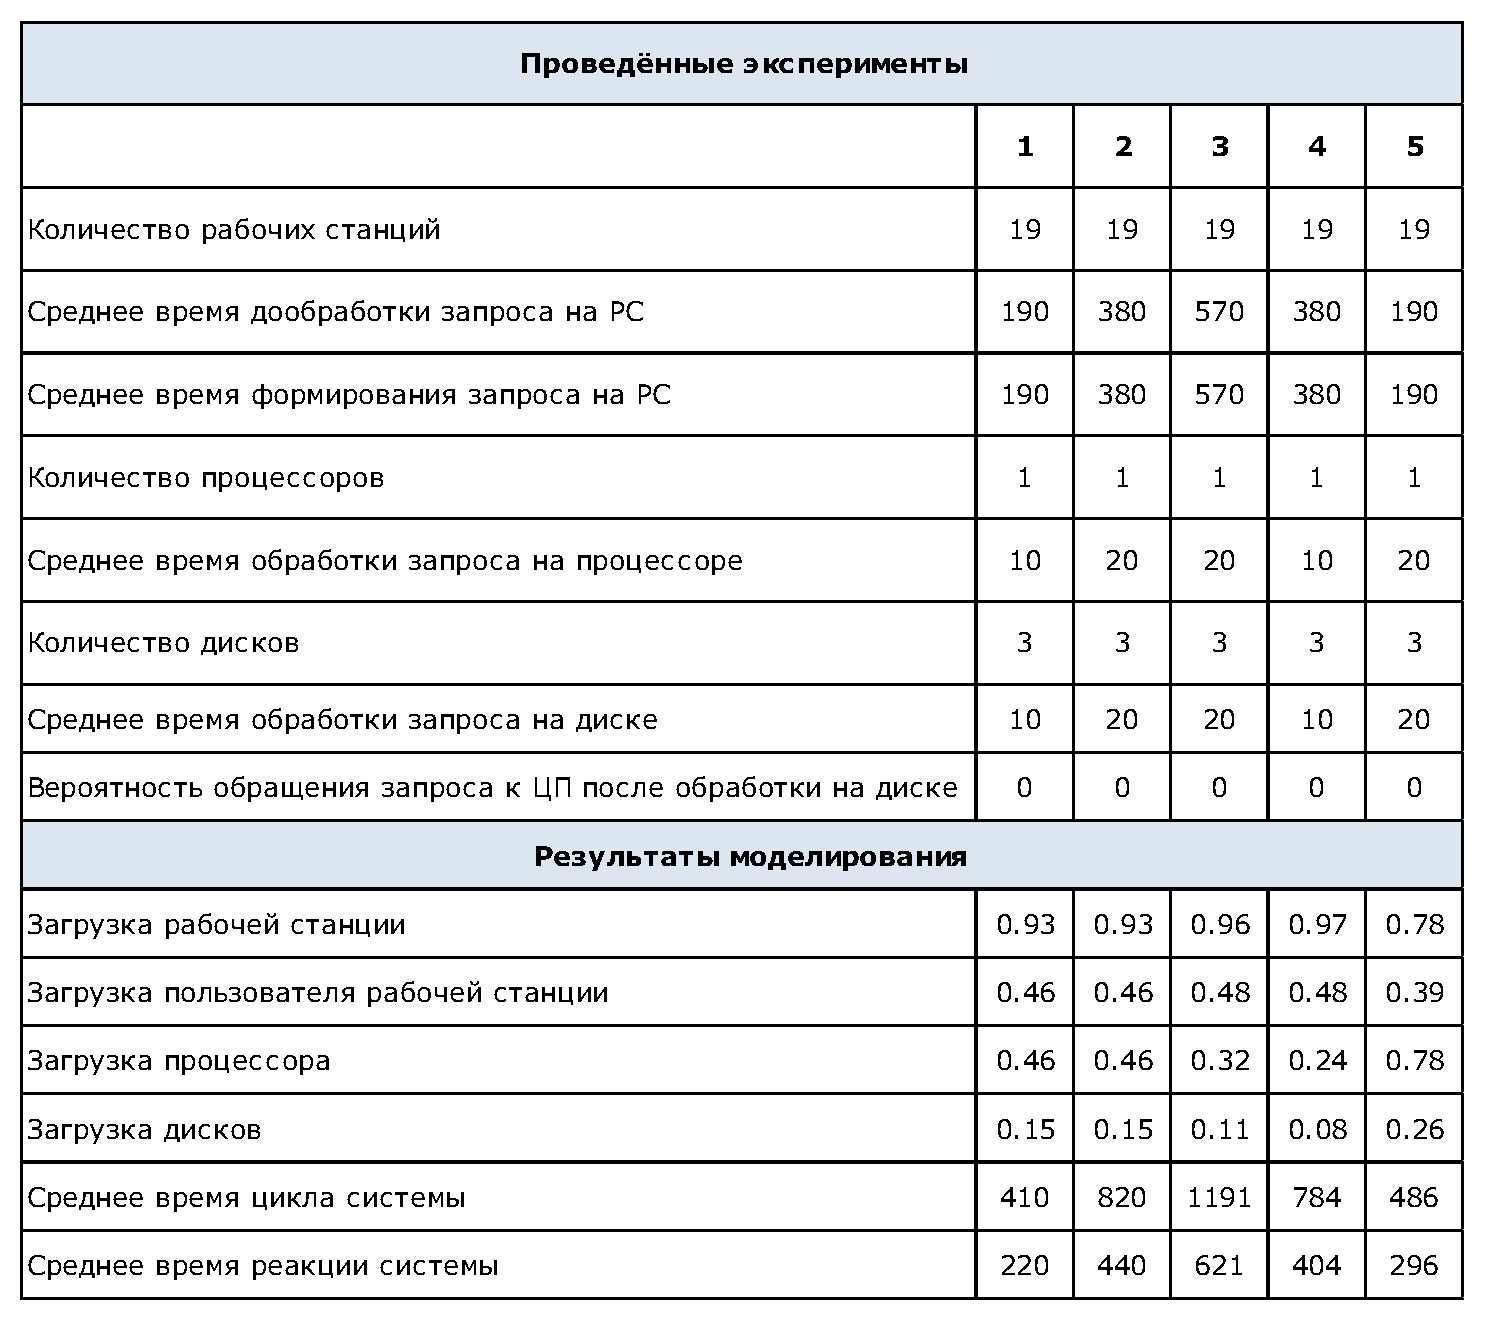
\includegraphics[width=0.7\linewidth]{pics/pic10_1_anal_result.eps}
 \end{tabular}
\end{table}